\begin{table}[h]
    \centering
    \caption{Comparação do Tempo do Bubble Sort}
    \begin{tabular}{|c|c|c|c|c|c|c|}
        \hline
        Tamanho de Entrada & 10 & 100 & 1000 & 10000 & 100000 & 1000000 \\
        \hline
        Crescente & 0.000000 & 0.000000 & 0.001000 & 0.098000 & 9.734000 & 952.523000 \\
        \hline
        Decrescente & 0.000000 & 0.000000 & 0.002000 & 0.172000 & 17.373000 & 1697.082000 \\
        \hline
        Aleatória & 0.000000 & 0.000000 & 0.001000 & 0.212000 & 25.232000 & 2665.916000 \\
        \hline
    \end{tabular}
    \label{tab:comparacaobubble}
\end{table}

A Tabela \ref{tab:comparacaobubble} mostra o Bubble Sort nos 6 diferentes tamanhos
de entrada e 3 situações diferentes de como as entradas são postas em determinados arquivos, assim como os demais algoritmos.Os resultados evidenciaram certas características fundamentais do algoritmo Bubble Sort. Este algoritmo exibe uma performance uniforme e estável, gerando resultados semelhantes em diversas condições de entrada. O Bubble Sort, devido à sua abordagem de comparação e troca sequencial, não se beneficia substancialmente de dados parcialmente ordenados e, consequentemente, sua eficiência é consideravelmente constante, independentemente do estado inicial dos dados, mesmo com esse resultado ele ter demorado mais na forma aleatória, o médio caso dele possui a mesma complexidade dos demais.


\begin{figure}[h!]
    \centering
    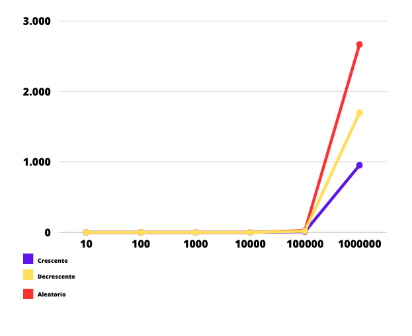
\includegraphics[width = 10cm]{Imagens/Bubble Sort/Captura de tela 2023-09-27 211808.png}
    \caption{Gráfico de tempo do algoritmo Merge Sort.}
    \label{fig:b10}
\end{figure}